\subsection{URL dispatching}

Orice aplicatie care distribuie informatia sub forma unor pagini web are un sistem de traducere a solicitarilor clientilor (URL) catre elemente executabile din interior. 

Schema de URL-uri corespunzatoare controller-elor care servesc interfata de administrare a aplicatiei este descrisa in figura urmatoare. 
Pornind de la un URL de forma http://<server>:8080/admin/<cerere>{/{id} | ?param=val}, se poate observa modul general in care aplicatia raspunde unei solicitari formulate in acest mod.

\bigskip

\begin{center}
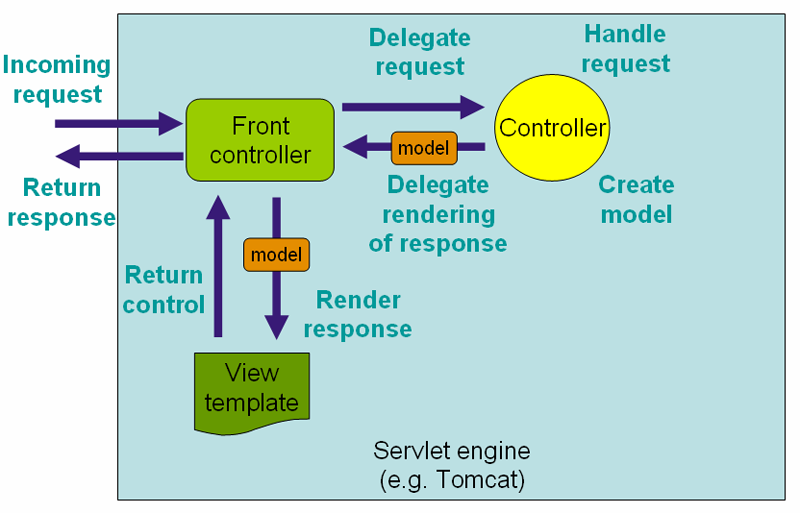
\includegraphics[width=\textwidth]{mvc.png}
\end{center}

\bigskip

\begin{center}
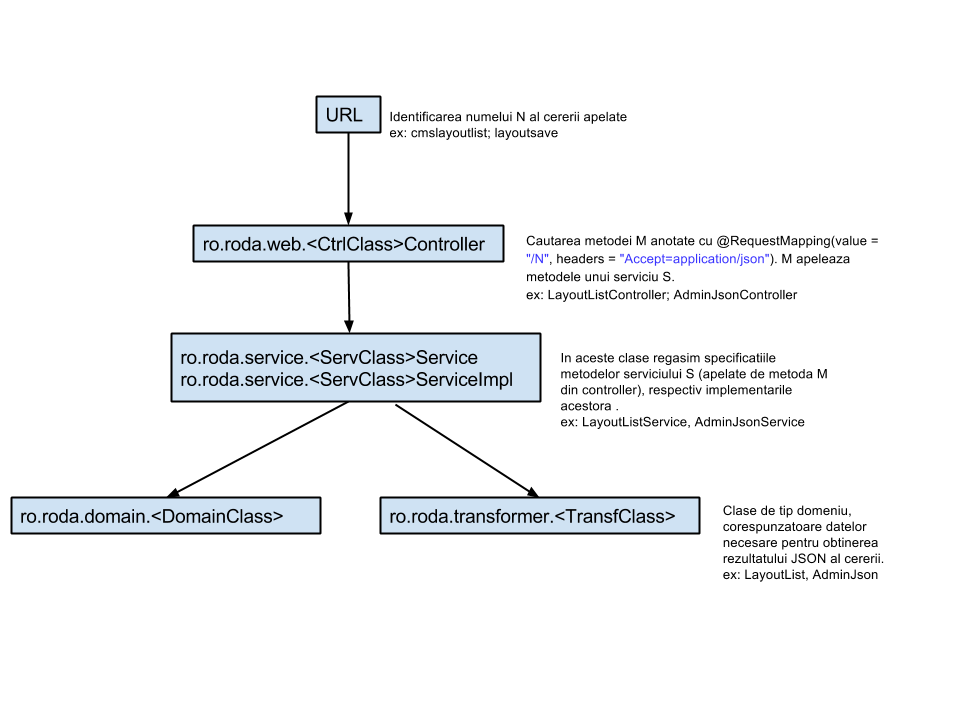
\includegraphics[width=\textwidth]{roda_URL.png}
\end{center}

\bigskip

